\chapter{Modello}

\section{Ambiente costruito}

Prima di andare a definire gli agenti che operano nel nostro modello, abbiamo raccolto informazioni sulla possibile struttura dell'ambiente di un pronto soccorso, al fine di costruire una piantina che avesse le caratteristiche generiche di un pronto soccorso comune. 

In particolare, le stanze che abbiamo infine deciso di realizzare sono le seguenti: 
\begin{itemize}
    \item Sala d'attesa
    \item Accettazione: 2 file
    \item Triage: 2 stanze
    \item Sala visita: 4 stanze
    \item Chirurgia: 2 sale operatorie
    \item Degenza breve: 1 con posti letto normali, 1 con posti letto di emergenza
\end{itemize}

\begin{figure}[!htb]
    \centering
    \makebox[\textwidth][c]{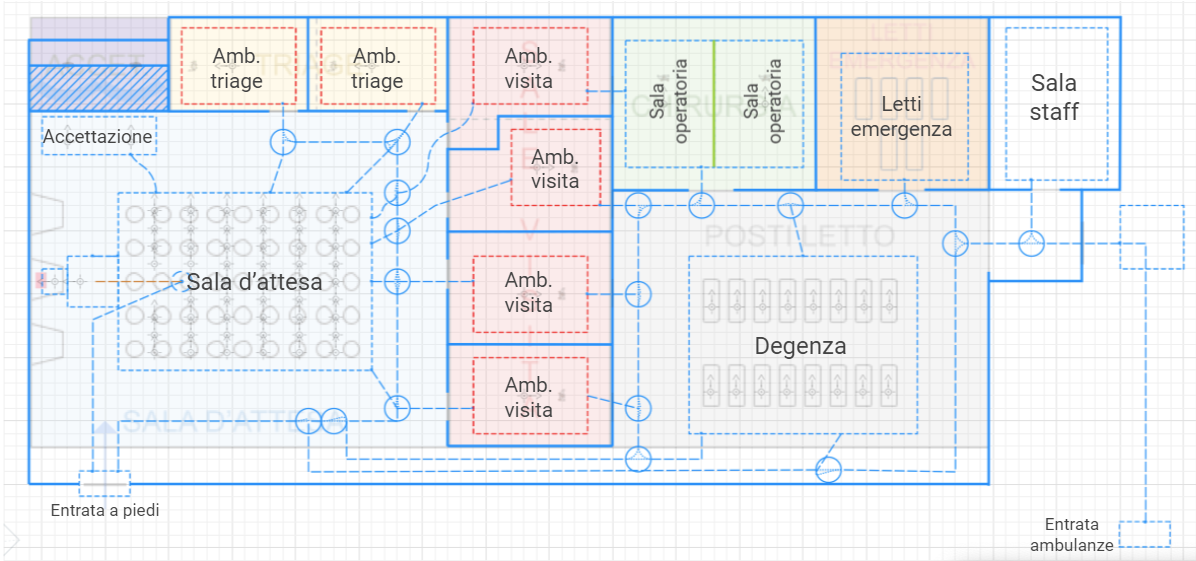
\includegraphics[width=1\textwidth]{layout}}   
    \caption{Layout 2D dell'ambiente costruito}
    \label{fig:layout}
\end{figure}
\begin{figure}[!htb]
    \centering
    \makebox[\textwidth][c]{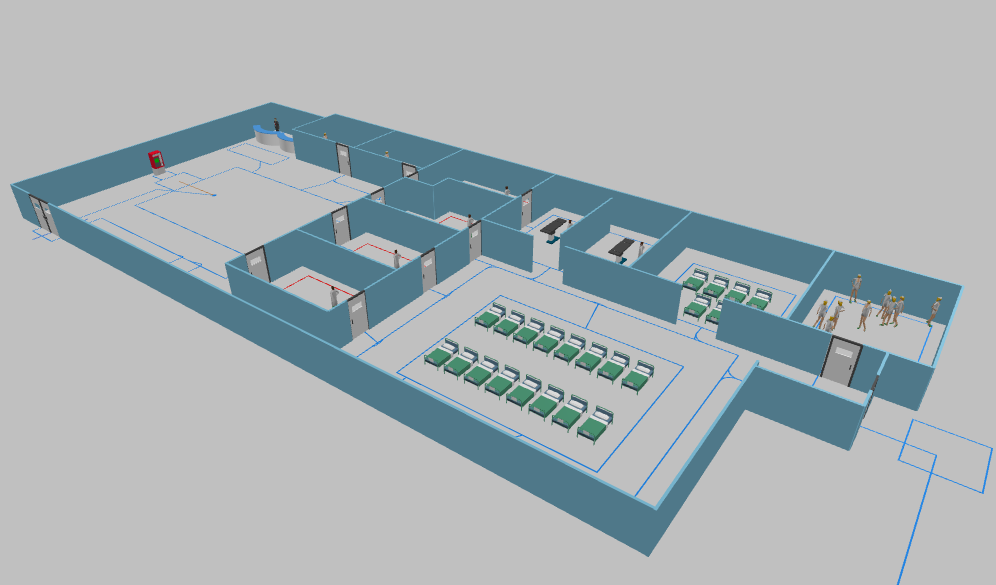
\includegraphics[width=1\textwidth]{3d presentation}}   
    \caption{Layout 3D dell'ambiente costruito}
    \label{fig:layout3D}
\end{figure}

\section{Agenti realizzati}

Gli agenti che abbiamo realizzato per impostare il funzionamento del modello sono Patient, Ambulance, AmbulancePatient e Nurse. 
Mentre i primi tre sono generati in base ad uno specifico tasso di input, gli infermieri appartengono ad una pool di risorse per cui vengono effettuate delle richieste all'occorrenza.

\subsection{Patient}

Questo agente è il più importante del modello: rappresenta infatti il paziente che si reca al pronto soccorso. E' caratterizzato da alcuni parametri che ne definiscono il comportamento all'interno del workflow: 

\paragraph{\textit{appearance}}
Definisce l'agente a livello puramente estetico tramite un'estrazione da una distribuzione uniforme discreta, con tre possibili opzioni.  

\paragraph{\textit{priority}}
Definisce tramite un numero intero la priorità di ogni paziente, data la gravità della sua situazione e rispetto agli altri pazienti che sono arrivati; viene impostato a zero nel momento della creazione dell’agente e verrà modificato durante il triage, sulla base del parametro \textit{sickness}.

\paragraph{\textit{sickness}}
È un parametro di tipo Illness, ovvero una Option List che contiene al suo interno le tipologie di urgenze (rosso, giallo, verde o bianco) e viene istanziato secondo una distribuzione ad hoc (\textit{IllnessDistr}), che segue un andamento pressoché realistico: 
\begin{itemize}
    \item Codice rosso: $10\%$ dei pazienti
    \item Codice giallo: $25\%$ dei pazienti
    \item Codice verde: $40\%$ dei pazienti
    \item Codice rosso: $25\%$ dei pazienti
\end{itemize}

\paragraph{\textit{surgery}}
È un parametro di tipo NeedSurgery, ovvero una Option List (con opzioni \textit{yes} oppure \textit{no}) che descrive il bisogno o meno di ricorrere alla chirurgia per un determinato paziente.

\paragraph{\textit{bed}}
È un parametro di tipo NeedBed, ovvero una Option List (con opzioni \textit{yesB} oppure \textit{noB}) che viene utilizzato per segnalare la necessità di un letto per il paziente.

\paragraph{\textit{hospital}}
È un parametro booleano che viene impostato a \textit{true} quando il periodo di degenza supera le 20 ore: in questo caso il paziente viene immediatamente trasferito in ospedale. 

\paragraph{\textit{newVisit}}
È un parametro booleano che viene impostato a \textit{true} quando un paziente ha bisogno di un'ulteriore visita in seguito ad un periodo in degenza. 

\paragraph{\textit{leave, leaveProb, leaveEst()}}
Rispettivamente un parametro, una variabile ed una funzione che permettono di implementare il meccanismo di noia durante l’attesa e conseguente uscita volontaria dal PS (meccanismo descritto nel seguito).

\paragraph{\textit{cameByAmb}}
È un parametro booleano che definisce se il paziente è arrivato in ambulanza o meno. Tale valore è importante poiché permette di definire la transizione dallo stato \textit{initial} allo stato \textit{other}, possibile solamente per i pazienti che arrivano in ambulanza e non hanno dunque bisogno di aspettare in sala d'attesa.

\paragraph{\textit{entryTime, waitingEntryTime, waitingTime}}
Sono variabili di tipo double che permettono di definire il tempo (inteso come timestamp) di entrata del paziente, di entrata nello stato \textit{Waiting} e il tempo che passa in quest'ultimo. 
Sono utili perlopiù per definire le statistiche descritte nel capitolo \ref{chap:sper}. 

\subsubsection{Meccanismo di uscita volontaria}
All’interno dei pronto soccorso, date le elevate attese, molti pazienti scelgono di andarsene prematuramente. Essendo quindi una situazione possibile ed ampiamente frequente abbiamo deciso di dotare ogni agente di questa peculiarità che può portarli o meno ad abbandonare prematuramente l’ospedale, sfruttando la possibilità offerta da AnyLogic che permette di implementare diagrammi di stato all'interno delle classi che rappresentano gli agenti. 

In questi diagrammi, ogni blocco identifica uno stato in cui l’agente può trovarsi: nello specifico, un agente di tipo Patient si trova inizialmente nello stato Initial, da cui passa in Waiting a condizione che l’agente si trovi nella sala d’attesa. 

L’agente rimane in questo stato finché non viene visitato oppure se viene chiamato (accettazione, triage, visita, che gli permettono di passare nello stato Other); se invece non viene chiamato entro 60 minuti, passa nello stato WantsToLeave, al cui ingresso viene valutata la decisione di andarsene (parametro leave) tramite la funzione leaveEst(), con una probabilità del 15\% (definita tramite la costante leaveProb). 

Nel caso in cui l’agente decidesse di non andarsene, dopo altri 30 minuti, se ancora in attesa, invocherà nuovamente la funzione di decisione.  

Nello stato Leaving il paziente si accingerà a muoversi verso la porta di uscita; nello stato Left, eliminerà se stesso dall’ambiente. 

C’è infine la possibilità che un paziente precedentemente nello stato Other ritorni in WantsToLeave nel caso in cui si trovasse ancora una volta in sala d’attesa. 

\begin{figure}[!htb]
    \centering
    \makebox[\textwidth][c]{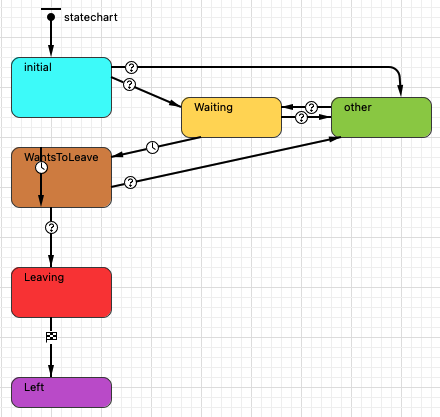
\includegraphics[width=300px]{patientStatechart}}   
    \caption{\textit{Statechart} dell'agente Patient}
    \label{fig:statechart}
\end{figure}

\subsection{Ambulance e AmbulancePatient}

Ambulance e AmbulancePatient sono le due classi di agenti definite per rappresentare i pazienti che giungono al pronto soccorso in ambulanza. Nell'ambiente hanno un'entrata prioritaria che permette loro di saltare le fasi di accettazione, triage e visita. 

Ambulance è definito ai fini del modello solo come mezzo di trasporto "contenitore" per i pazienti di tipo AmbulancePatient.
Viene generato uno di questi agenti all'occorrenza, ovvero quando un agente di tipo AmbulancePatient ha bisogno di essere trasportato in ambulanza fino al pronto soccorso. 

AmbulancePatient è un'estensione della classe che definisce l'agente Patient e mantiene dunque i suoi parametri descritti in precedenza; per questo agente viene però impostato di default il bisogno di un letto per la degenza, mentre gli altri parametri sono impostati come segue nel blocco di generazione: 
\begin{itemize}
    \item Priority: il valore viene generato da una distribuzione uniforme discreta con valori compresi tra 6 e 10. 
    \item Surgery: viene impostato un valore casuale tra yes e no. 
    \item Sickness: per gli arrivi in ambulanza viene sempre impostato a Red. 
\end{itemize}

\subsection{Nurse}
È l'agente che rappresenta gli infermieri: questi sono generati nel modello in un numero variabile in base all'impostazione del pool di risorse che li contiene. 
La classe che definisce l'agente non presenta parametri, funzioni o stati particolari ma serve a definire solo a livello estetico gli infermieri. 
Questi agenti sono utilizzati nel workflow del sistema esclusivamente tramite blocchi di tipo \textit{seize} e \textit{release}, che permettono di "riservarli" per un tempo utile ad eseguire una determinata azione (nel nostro caso, accompagnare i pazienti in varie stanze qualora ce ne sia bisogno). 

\section{Workflow}

Il workflow è la parte focale della costruzione del sistema tramite il software AnyLogic e viene mostrato interamente nella figura \ref{fig:wf-all}.
\\Permette infatti di far interagire agenti ed ambiente secondo determinate regole e condizioni, che possono essere specificate tramite la modellazione a blocchi e, per ciascun blocco, estese con linguaggio Java. 

In questa sezione verrà descritta ogni fase del workflow realizzato, al fine di far comprendere al lettore non solo il funzionamento del modello in sè, ma anche quali sono alcune delle funzionalità offerte da Anylogic. 

\begin{figure}[!htb]
    \centering
    \makebox[\textwidth][c]{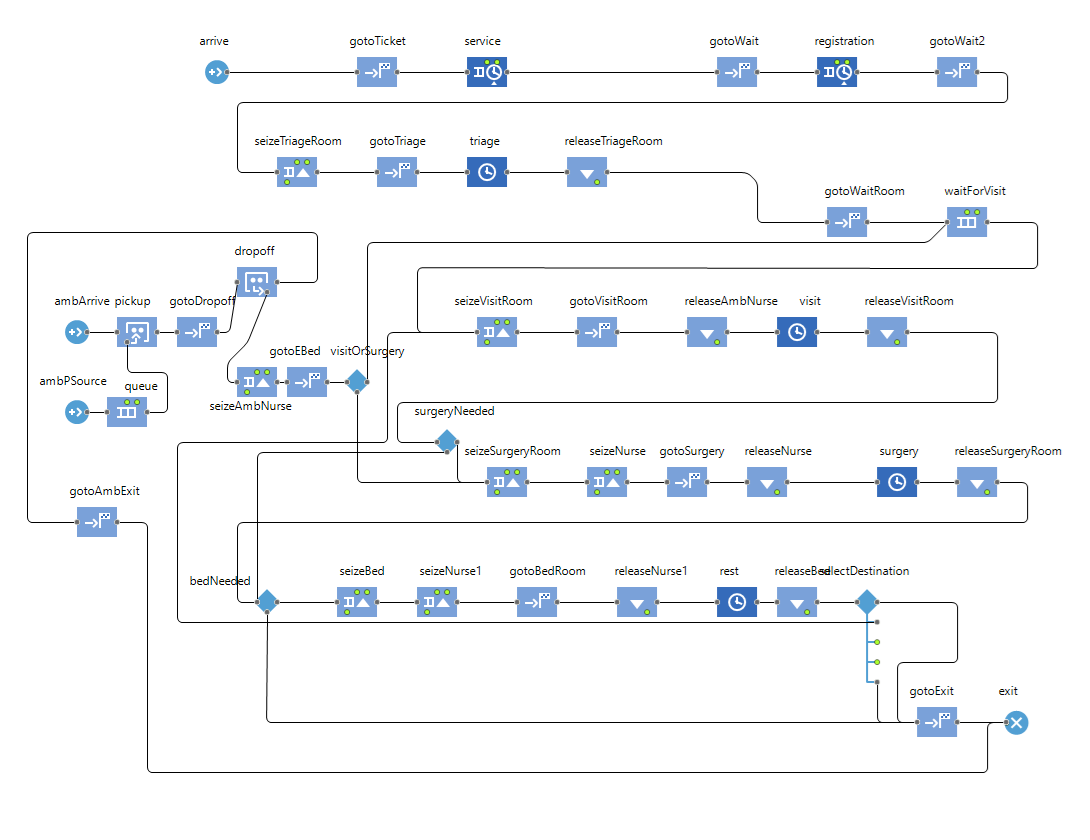
\includegraphics[width=1\textwidth]{workflow/wf-all}}   
    \caption{Workflow complessivo del sistema}
    \label{fig:wf-all}
\end{figure}

\clearpage
\subsection{Strumenti utilizzati nel Workflow} \label{chap:param}
Nell’implementazione della simulazione abbiamo avuto necesità di utilizzare degli strumenti, tra cui le \textit{resource pool} che ci hanno permesso di definire degli insiemi di unità che potevano essere riservate (\textit{seized}) e rilasciate (\textit{released}) dagli agenti che utilizzavano i seguenti tipi di blocco: \texttt{Seize}, \texttt{Release}, \texttt{Delay} e \texttt{Service}.

In particolare abbiamo definito i seguenti insiemi: infermieri, biglietteria, accettazione (Registrars), triage, sala visita, chirurgia e letti disponibili.

\begin{figure}[!htb]
    \centering
    \makebox[\textwidth][c]{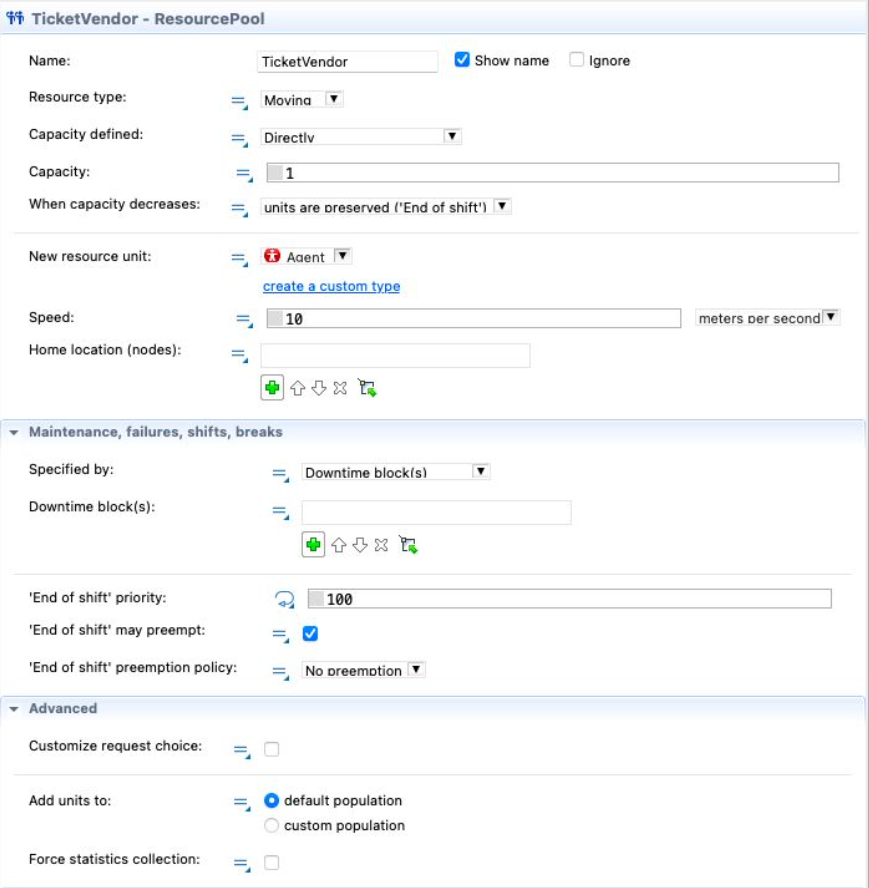
\includegraphics[width=350px]{Immagini/workflow/ResourcePool.png}}   
    \caption{Interfaccia Resource Pool}
\end{figure}

\clearpage
All'interno della simulazione è stato necessario inserire parametri e funzioni; i primi ci hanno permesso di definire delle caratteristiche statiche e le seconde sono state fondamentali per calcolare valori a runtime a seconda del percorso seguito dal paziente.  

All’interno del nostro \textit{Main} possiamo trovare tre funzioni e due parametri:
\begin{itemize}
\item \texttt{arrivalRate}: il numero di pazienti che arrivano per ora, che nel nostro caso è settato a 8 pazienti/ora.
\item \texttt{ambulanceArrRate}: il numero di pazienti che arrivano in ambulanza ogni ora (default 4 pazienti/ora). \\
\item \texttt{staffSpeed}: restituisce la velocità dello staff del pronto soccorso.
\item \texttt{patientSpeed}: restituisce  la velocità dei pazienti.
\item \texttt{restTime}: permette di calcolare il tempo che i pazienti necessitano di passare a letto, in base alla priorità assegnata.\\
\end{itemize}

\begin{figure}[!htb]
    \centering
    \makebox[\textwidth][c]{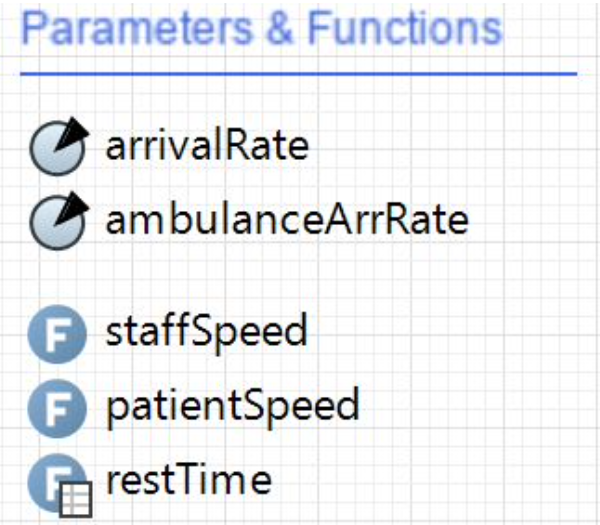
\includegraphics[width=200px]{Immagini/workflow/param.png}}   
    \caption{Parametri e Funzioni implementati}
\end{figure}
\clearpage
\subsection{L'arrivo del paziente}

Il nostro workflow ha due diversi punti d’inizio: il primo che andremo a trattare è il caso in cui il paziente arriva all'ospedale autonomamente, deve prendere il biglietto per poter sedersi in sala d’aspetto e successivamente essere chiamato per l’accettazione. Nel paragrafo \ref{chap:ambulance}  verrà trattato anche il caso in cui il paziente arrivi trasportato in ambulanza.

Questa parte del workflow comprende il blocco \texttt{arrive} da cui tutto il workflow ha inizio. All'interno di essp è possibile definire il rate di arrivo degli agenti (parametro \texttt{arrivalRate}) e la velocità che avranno nel modello (funzione \texttt{patientSpeed()}). 
Inoltre in questo blocco,  come in tutti quelli successivi, è possibile definire la zona della simulazione in cui avviene l’azione e quale agente specifico è coinvolto (Patient in questo caso). 

Il paziente arriva e va a prendere il biglietto con il blocco di movimento \texttt{gotoTicket} che segnala all’agente in che punto della simulazione recarsi.

Il blocco successivo \texttt{service} invece è quello designato per prendere il biglietto che sarà necessario per aspettare il turno dell’accettazione nella sala d’aspetto.\\ Questo blocco è particolare in quanto permette di prendere delle risorse da una \texttt{resource pool} (Ticket Machine), creare una coda di grandezza prestabilita e settare un delay: per entrambe le cose è possibile definire il nodo in cui le azioni devono avvenire. 

Dopo che l’agente ha preso il numero, con il blocco di movimento \texttt{gotoWait} si sposta in sala d’aspetto fino a che non verrà chiamato per effettuare l'accettazione.

\begin{figure}[!htb]
    \centering
    \makebox[\textwidth][c]{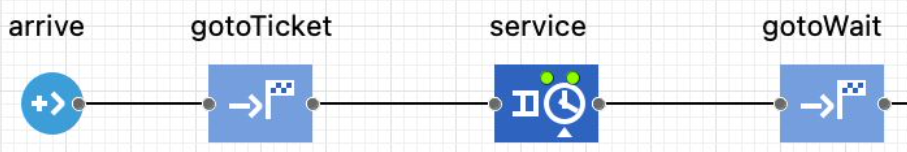
\includegraphics[width=1\textwidth]{Immagini/workflow/patient-arrive.png}}   
    \caption{Workflow dell'arrivo del paziente}
\end{figure}

\clearpage
\subsection{Triage}
L’agente entra nel blocco \texttt{registration} che preleva una persona, se libera, dalla resource pool \texttt{Registrars} che avrà il compito di fare l’accettazione al paziente (ne sono presenti due); inoltre è settato un delay secondo una distribuzione triangolare, che sarà il tempo impiegato per effettuare l’accettazione. \\ Infine, vengono delineate due zone: quella per aspettare in coda che l’accettazione sia libera e la zona in cui effettivamente effettuarla.\\ Dopo che il paziente effettua l’accettazione, tramite il blocco di movimento \texttt{gotoWait2} torna in sala d’aspetto.

Il blocco successivo \texttt{seizeTriageRoom} crea la coda di persone che nella \texttt{WaitingRoom} aspettano di venir chiamati per andare a fare il triage, richiede alla resource pool \texttt{TriageRooms} se ci sia una sala libera e nel caso ci fosse la riserva per il paziente; tramite il blocco \texttt{gotoTriage} l’agente ci si dirige, altrimenti rimane nella coda ad aspettare una sala libera.

Il triage viene eseguito dal blocco \texttt{triage} che ha la particolarità di creare un delay in cui verosimilmente viene effettuato un triage: da questo blocco il paziente uscirà con la diagnosi e gli verrà assegnata una priorità.

Alla fine di queste operazioni, tramite il blocco \texttt{release TriageRoom} 
viene liberata la sala per il triage 
che ritornerà disponibile nella resource pool \texttt{TriageRooms}.\\


\begin{figure}[!htb]
    \centering
    \makebox[\textwidth][c]{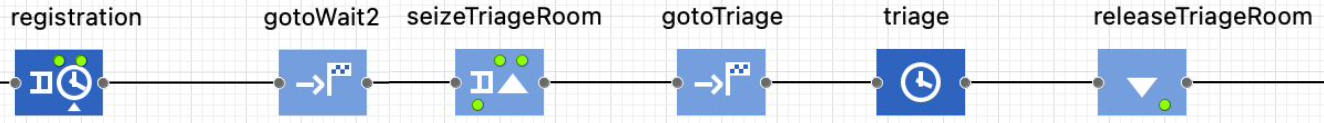
\includegraphics[width=1\textwidth]{Immagini/workflow/triage.png}}   
    \caption{Workflow del triage}
\end{figure}

\clearpage

\subsection{Visita Specialistica}
La priorità affidata al paziente sulla base della diagnosi sarà la discriminante per mandarlo direttamente alle sale visita (in casi di codice rosso) oppure ad aspettare in sala d’attesa.

Nel caso in cui il paziente non è troppo grave viene quindi mandato nella sala d’attesa (\texttt{gotoWaitRoom}) e si mette in fila (\texttt{wairForVisit}), quest'ultima gestita secondo una politica priority-based (a seconda della priorità di ciascun paziente).

Quando il paziente è il primo della coda, viene controllato se nella resource pool \texttt{VisitRooms} vi sia una sala visita libera e nel caso vi sia viene mandato a fare la visita (\texttt{gotoVisitRoom}).
 
Durante la visita viene valutato se sia necessaria la chirurgia e/o un letto. Al termine della visita viene 
rilasciata la sala visita (\texttt{releaseVisitRoom}) che torna nella resource pool \texttt{VisitRooms}. \\


\begin{figure}[!htb]
    \centering
    \makebox[\textwidth][c]{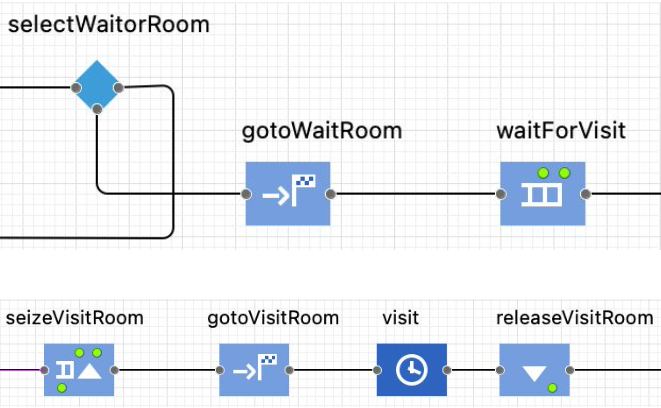
\includegraphics[width=250px]{Immagini/workflow/visit.png}}   
    \caption{Workflow di una visita specialistica}
\end{figure}

\clearpage
\subsection{Chirurgia}  
Nel caso in cui il paziente avesse bisogno di un intervento in chirurgia (\texttt{surgeryNeeded}) viene verificato che ci siano delle sale operatorie (\texttt{seize SurgeryRoom}) e 
infermieri (\texttt{seizeNurse}) liberi.
\\ Se queste due condizioni sono verificare il paziente viene spostato in chirurgia con l'aiuto dell’infermiere (\texttt{gotoSurgery}) che viene rilasciato (\texttt{releaseNurse}) nel momento in cui il paziente arriva nella sala, tornando al nodo \texttt{staffRoom}. \\
L’intervento (\texttt{surgery}) dura per un tempo variabile che segue una distribuzione triangolare e nel momento in cui finisce la sala viene liberata (\texttt{release SurgeryRoom}).


\begin{figure}[!htb]
    \centering
    \makebox[\textwidth][c]{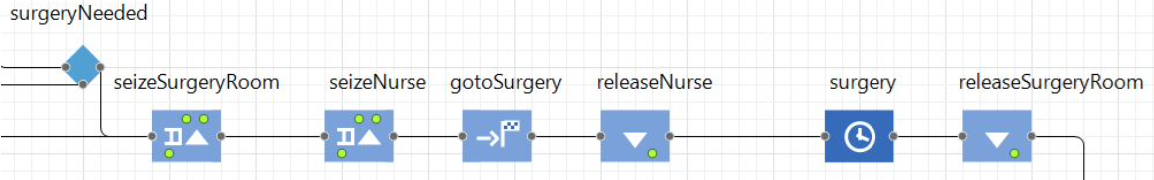
\includegraphics[width=1\textwidth]{Immagini/workflow/chirurgia.png}}   
    \caption{Workflow di un intervento chirurgico}
\end{figure}

\subsection{Degenza e uscita}  
Il paziente può aver bisogno di un letto in due casi: se ha avuto un intervento chirurgico oppure ha bisogno di essere genericamente monitorato. 

Viene quindi controllato che ci siano un letto disponibile (\texttt{seizeBed}) e un infermiere libero (\texttt{seizeNurse1}) per accompagnare il paziente nella degenza (\texttt{gotoBedRoom}), infermiere che torna a disposizione dopo aver portato il paziente (\texttt{releaseNurse1}).

Durante la degenza (\texttt{rest}) i pazienti possono aver bisogno di ulteriori visite (seconda uscita del blocco \texttt{selectDestination}) oppure i problemi possono risolversi ed essere dimessi (prima e ultima uscita, ovvero quella di default). Dopo un delay variabile a seconda della gravità del paziente questo parametro viene aggiornato.

Nel caso in cui non fosse necessaria un’ulteriore visita il paziente può uscire (\texttt{gotoExit}) liberando il letto (\texttt{releaseBed}).


\begin{figure}[!htb]
    \centering
    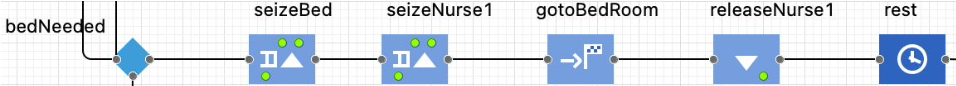
\includegraphics[width=1\textwidth]{Immagini/workflow/bed1.png}
\end{figure}
\begin{figure}[!htb]
    \centering
    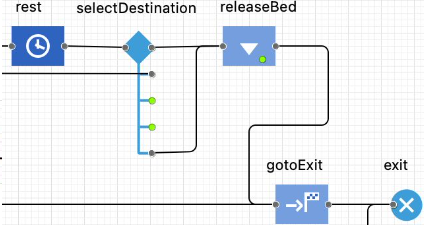
\includegraphics[width=220px]{Immagini/workflow/bed2.png} 
    \caption{Workflow della degenza e dll'uscita}
\end{figure}

\subsection{Arrivo in Ambulanza} \label{chap:ambulance}

Un paziente oltre a poter arrivare al pronto soccorso da solo può arrivare in ambulanza.

Le ambulanze vengono generate dal blocco \texttt{ambArrive} ogni qualvolta un paziente ha bisogno del loro intervento.

I pazienti bisognosi vengono creati dal blocco \texttt{ambPSource}, dal quale poi vengono inviati in una coda per attendere l’arrivo dell’ambulanza. All’entrata nel blocco di coda, viene invocata la funzione \texttt{inject()} sul blocco di generazione delle ambulanze per chiamarne una all’occorrenza. 

L’ambulanza funge da container e  tramite il blocco \texttt{pickup} carica il paziente e lo scarica (tramite \texttt{dropoff}) all’entrata per ambulanze del pronto soccorso, dove gli viene riservato un infermiere per portarlo ad effettuare una visita o, nei casi più urgenti, una chirurgia.

\begin{figure}[!h]
    \centering
    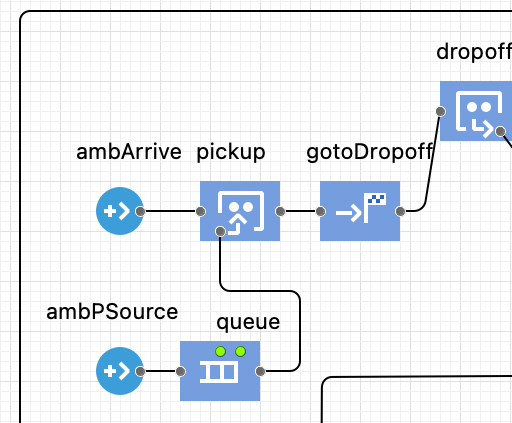
\includegraphics[width=250px]{Immagini/workflow/Ambulance.png} 
    \caption{Workflow dell'arrivo in ambulanza}
\end{figure}



